\newpage
\rhead{\textbf{\textcolor{blue}{Т}\textcolor{gray}{ерминология: Информация и данные}}}
\begin{tikzpicture}[remember picture,overlay]
    \node[anchor=north west,yshift=-1.5pt,xshift=1pt]%
        at (current page.north west)
        {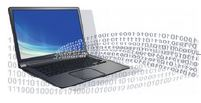
\includegraphics[scale=0.5]{pic_1} };
\end{tikzpicture}

\vskip 0.5cm

\newline
\begin{flushleft}
 Международный стандарт ISO/IEC 2382:2015\\
«Information technology – Vocabulary» (вольный пересказ):\\
\qquad \textcolor{Green}
{Информация} – знания относительно фактов, событий, \\ \qquad вещей, идей и  понятий.
\\
		\qquad \textcolor{Green}{Данные} – форма представления информации в виде, \\ \qquad пригодном для передачи или обработки. \\
\end{flushleft}
	\vspace*{3mm}
	\textbullet \ Что есть предмет информатики: информация или данные? \\
	\textbullet \ Как измерить информацию? Как измерить данные? 	Пример: «Байкал — самое глубокое озеро Земли».